%%%%%%%%%%%%%%%%%%%% author.tex %%%%%%%%%%%%%%%%%%%%%%%%%%%%%%%%%%%
%
% sample root file for your "contribution" to a contributed volume
%
% Use this file as a template for your own input.
%
%%%%%%%%%%%%%%%% Springer %%%%%%%%%%%%%%%%%%%%%%%%%%%%%%%%%%%%%%%%%


%% RECOMMENDED %%%%%%%%%%%%%%%%%%%%%%%%%%%%%%%%%%%%%%%%%%%%%%%%%%%
%\documentclass[graybox]{svmult}
%
%% choose options for [] as required from the list
%% in the Reference Guide
%
%\usepackage{mathptmx}       % selects Times Roman as basic font
%\usepackage{helvet}         % selects Helvetica as sans-serif font
%\usepackage{courier}        % selects Courier as typewriter font
%\usepackage{type1cm}        % activate if the above 3 fonts are
                             % not available on your system
%
%\usepackage{makeidx}         % allows index generation
%\usepackage{graphicx}        % standard LaTeX graphics tool
%                             % when including figure files
%\usepackage{multicol}        % used for the two-column index
%\usepackage[bottom]{footmisc}% places footnotes at page bottom
%
%% see the list of further useful packages
%% in the Reference Guide
%
%\makeindex             % used for the subject index
%                       % please use the style svind.ist with
%                       % your makeindex program
%
%%%%%%%%%%%%%%%%%%%%%%%%%%%%%%%%%%%%%%%%%%%%%%%%%%%%%%%%%%%%%%%%%%%%%%%%%%%%%%%%%%%%%%%%%%
%
%\begin{document}

\title{Computational Fluid Dynamics - Wind}
% Use \titlerunning{Short Title} for an abbreviated version of
% your contribution title if the original one is too long
\author{
    \textbf{Ahsan Kareem}}
\tocauthor{}
\authorrunning{Kareem}
% Use \authorrunning{Short Title} for an abbreviated version of
% your contribution title if the original one is too long
%\institute{Name of First Author \at Name, Address of Institute, %\email{name@email.address}
%\and Name of Second Author \at Name, Address of Institute %\email{name@email.address}}
%
% Use the package "url.sty" to avoid
% problems with special characters
% used in your e-mail or web address
%
\maketitle

Buildings exposed to wind undergo complex interactions, which preclude a simple functional relationship between wind and its load effects with the exception of buffeting effects, i.e., turbulence excited wind loads along the direction of the wind. Accordingly, wind tunnels have traditionally served as a means of quantifying wind loads that are combined with structural analysis codes based on the finite-element analysis. 

With burgeoning growth in computational resources and parallel advances in computational fluid dynamics, computational simulations are evolving with the promise of becoming versatile, convenient, and reliable means of assessing wind-load effects. Figure \ref{fig:cfdWind_ExpCompCompare} summarizes salient advantages and disadvantages of the wind-tunnel-based experimental methods and the computational CFD-based schemes.

\begin{figure}[htb]
    \centering
    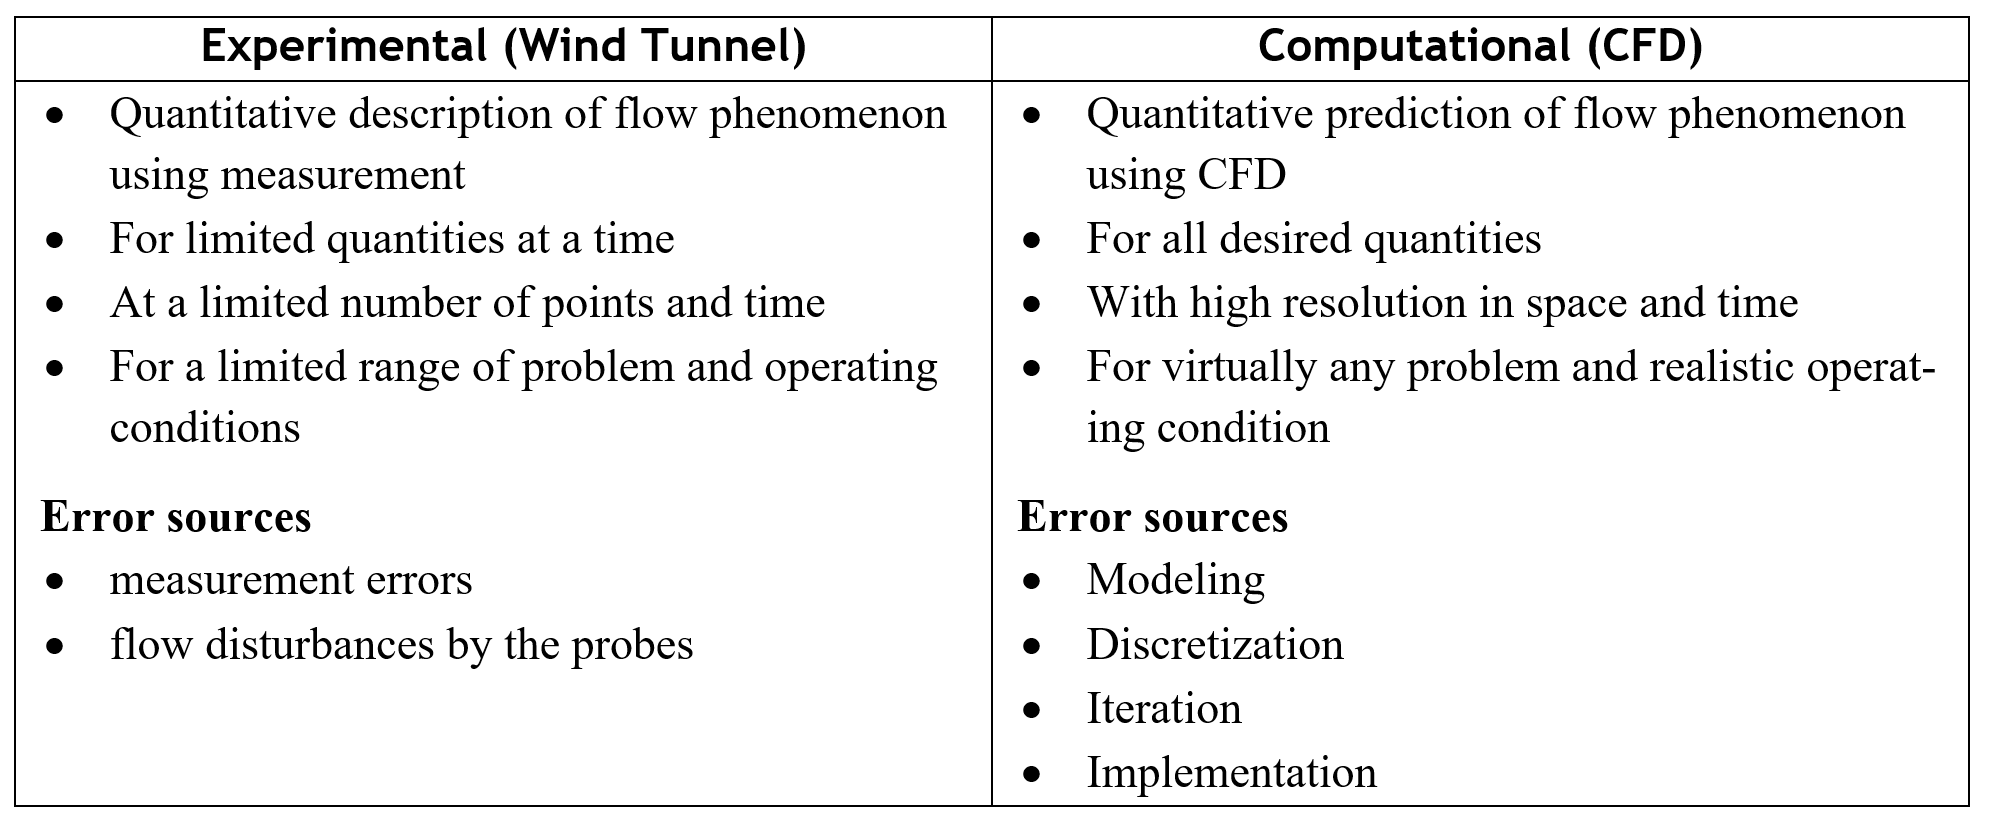
\includegraphics[width=1.0\textwidth, angle = 0]{Figures/ExpCompCompare.png}
    \caption{Comparison between experimental and computational approaches}
    \label{fig:cfdWind_ExpCompCompare}
\end{figure}

While developments in CFD as applied to a host of topics in basic fluid dynamics, aerospace, automotive, and urban aerodynamics are evolving at a fast pace, there has been rather limited research focus on the development of CFD-based tools and schema to advance the computational modeling of wind effects on structures. Limited commercial software has been widely utilized by both researchers and industry that, due to the inherent nature of modeling and parametric sensitivities and the lack of flexibility to improvise, has often led to observations that reflect large variability and on occasions depart from experimental observations. This has fueled the misleading impression that CFD is currently inadequate to fully capture wind-structure interactions. Yet the current state-of-the-art of CFD application in wind effects has led to the development of in-house tools wrapped around OpenFOAM, which have advanced to the stage that the Architectural Institute of Japan (AIJ) now permits the use of CFD in place of other approaches, e.g., wind-tunnel testing with the stipulation that the AIJ guidelines concerning 3D LES and inflow simulation are followed. At this junction, it is prudent to say that despite advances in CFD, simulation of wind-load effects using CFD still faces challenges; therefore, wind tunnels remain as an essential validation tool.
 
\section{Challenges of CFD}
\label{sec:resp_cfd_wind_challenges}

The computational grid of complex geometries and clusters of structures is fundamental to CFD as it represents the computational domain in which calculations are carried out at regular intervals to simulate the passage of time. The more compact the spatially discretized grid and the smaller the time step, the more accurate and realistic are the simulated results. Unfortunately, simply introducing initial and boundary conditions does not ensure a solution because the system being solved is nonlinear, and the interaction among terms of the governing equations leads to the generation of multiple scales. Accordingly, one of the primary challenges with CFD is the trade-off between accuracy and computational effort. The choice of turbulence modeling discussed in the following plays a critical role in the level of accuracy obtained and the computational effort required. 

In addition, the efficacy of CFD is still under debate, although it had been successfully implemented in aerospace engineering and wind tunnels to validate final designs. This is primarily due to the nature of structural shape in aerospace applications like an airfoil with a streamlined shape, resulting in a flow field around it that essentially stays attached to the surface, which can be numerically captured rather accurately.
Figure \ref{fig:cfdWind_ExpCompCompare} summarizes the flow field around a streamlined airfoil to a circular cylinder and progressing to a sharped-edged body representing a typical building or a bridge cross-section. In contrast, as we move from an airfoil towards a circular cylinder and a rectangular cross-section, the flow field around them gets progressively more complex as the flow cannot negotiate the sharp changes in direction as it moves around the body and hence jettisons away, creating separated flow characterized by flow reversal. Capturing these interacting features numerically poses challenges, which has led to slower progress in the application of CFD in wind-load assessments on structures. In the following, a basic overview of the issues surrounding flow features around structural configurations and the role of turbulence is presented including ensuing numerical challenges.

\begin{figure}[htb]
    \centering
    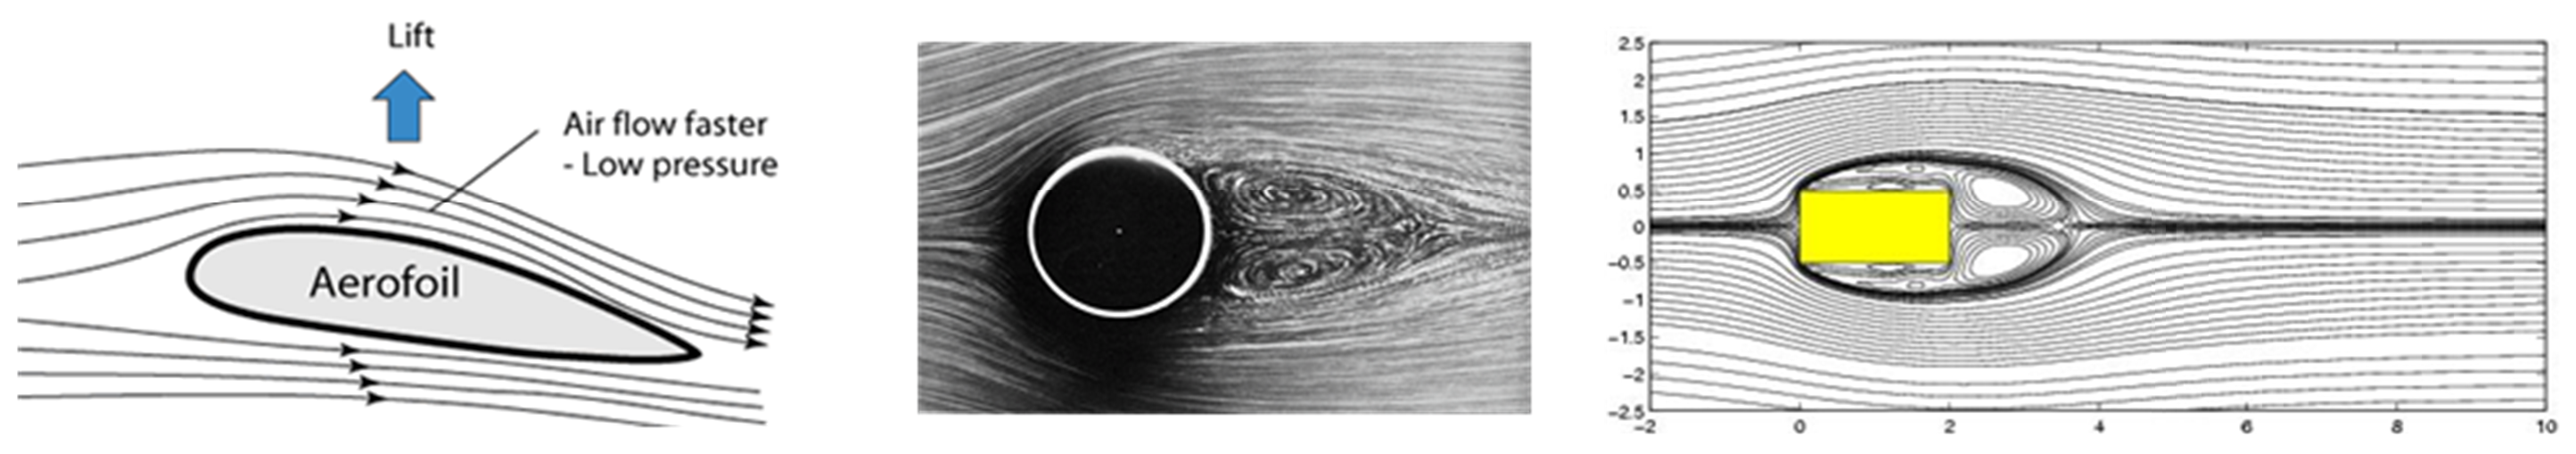
\includegraphics[width=1.0\textwidth, angle = 0]{Figures/FlowComplexity.png}
    \caption{Flow around cross-sections with increasing level of complexity \citep{ding2018aerodynamic}}
    \label{fig:cfdWind_ExpCompCompare}
\end{figure}

The range of the size of eddies that manifest the turbulent flow around structures determines the grid size, which places demands on both the memory size and speed of the computational hardware. Ideally, the resolution of all scales in the flow from energetic low-frequency fluctuations to the smallest scale (the Kolmogorov Scale) in the viscous dissipation regime dependent on viscosity would be ideal. This approach is referred to as direct numerical simulation (DNS) and is computationally very intensive as the grid size for a required Reynolds number (Re) flow requires cells equal to Re9/4. Although highly desirable, such simulations are currently limited to address basic research in fluid dynamics using CFD. 

To overcome this challenge, the NS equations of motion are filtered based on a length scale; thus, the motion of eddies smaller than the length scale is not calculated. Rather, the large eddy motion is computed, and the small-scale motions are modeled using ideas that range from enhanced coefficients of viscosity to an additional system of equations representing closure models. This results in a smoothing process, which helps to relax the number of grid points necessary to simulate the flow field. This scheme is known as the large eddy simulation (LES). As computer capacity increases, a broader range of eddies can be resolved, thus reducing the scales that need to be modeled. 

An alternative schema involves time averaging or ensemble averaging of the NS equations (the Reynolds averaging and referred to as RANS) that result in obtaining only the mean and deviations from the mean of the computed quantities. It requires a coarser grid resolution compared to LES. RANS often has difficulty in capturing flow separation and reattachment as a consequence of averaging \citep{spalart2010reflections}. The performance of LES may also be impaired with inadequate grid resolution and the treatment of the subgrid-scale turbulence. A hybrid combination of LES and RANS is referred to as detached eddy simulation (DES), composed of LES in regions for which the grid resolution can economically simulate the inertial subrange and reverts to RANS in near-wall regions where turbulence scale is smaller than the grid size \citep{hoarau2016progress}.

On the one hand, moving from the simulation of flow around isolated buildings to a cluster adds to the demand on computational resources; however, on the other hand, the flow patterns in the street canyons become more forgiving from the simulation perspective as sharply defined features become more unstructured due to mixing and can be resolved with less effort. Similar observations have been made in wind tunnel studies when examining the influence of adjoining buildings in a cluster on the aerodynamic loads. This is akin to adding damping in structures and helps to dampen fluctuations in the flow field. LES nested in weather research and forecasting models (WRF) models may be utilized to predict wind effects in a cluster of buildings in an urban setting under both extra-tropical and tropical systems. 

\section{Modeling of Flow around Structures}
\label{sec:resp_cfd_wind_flow_modeling}

The CFD simulation process for modeling wind around structures involves the following main steps: problem statement; mathematical model; mesh generation; space and time discretization; inflow generation; boundary conditions, wall functions, simulation runs, fluid-structure interaction (aeroelastic effects); post-processing; verification/validation; and uncertainty quantification. Some of the salient aspects are presented schematically in Figure \ref{fig:cfdWind_DAModeling}, with its primary focus on the choice of turbulence model, the mesh requirement especially near the boundaries of the structure, and inflow and boundary conditions \citep{ferziger2012computational}. Due to limitations in mesh resolution generally, it is essential to use a wall function. A wide variety of wall treatments for LES simulations of turbulent flows have been proposed (a recent overview is given in \citep{bose2018wall}, but the effect of the wall function formulation on the LES prediction of the turbulent pressure signal on a building has not been fully explored.

\begin{figure}[htb]
    \centering
    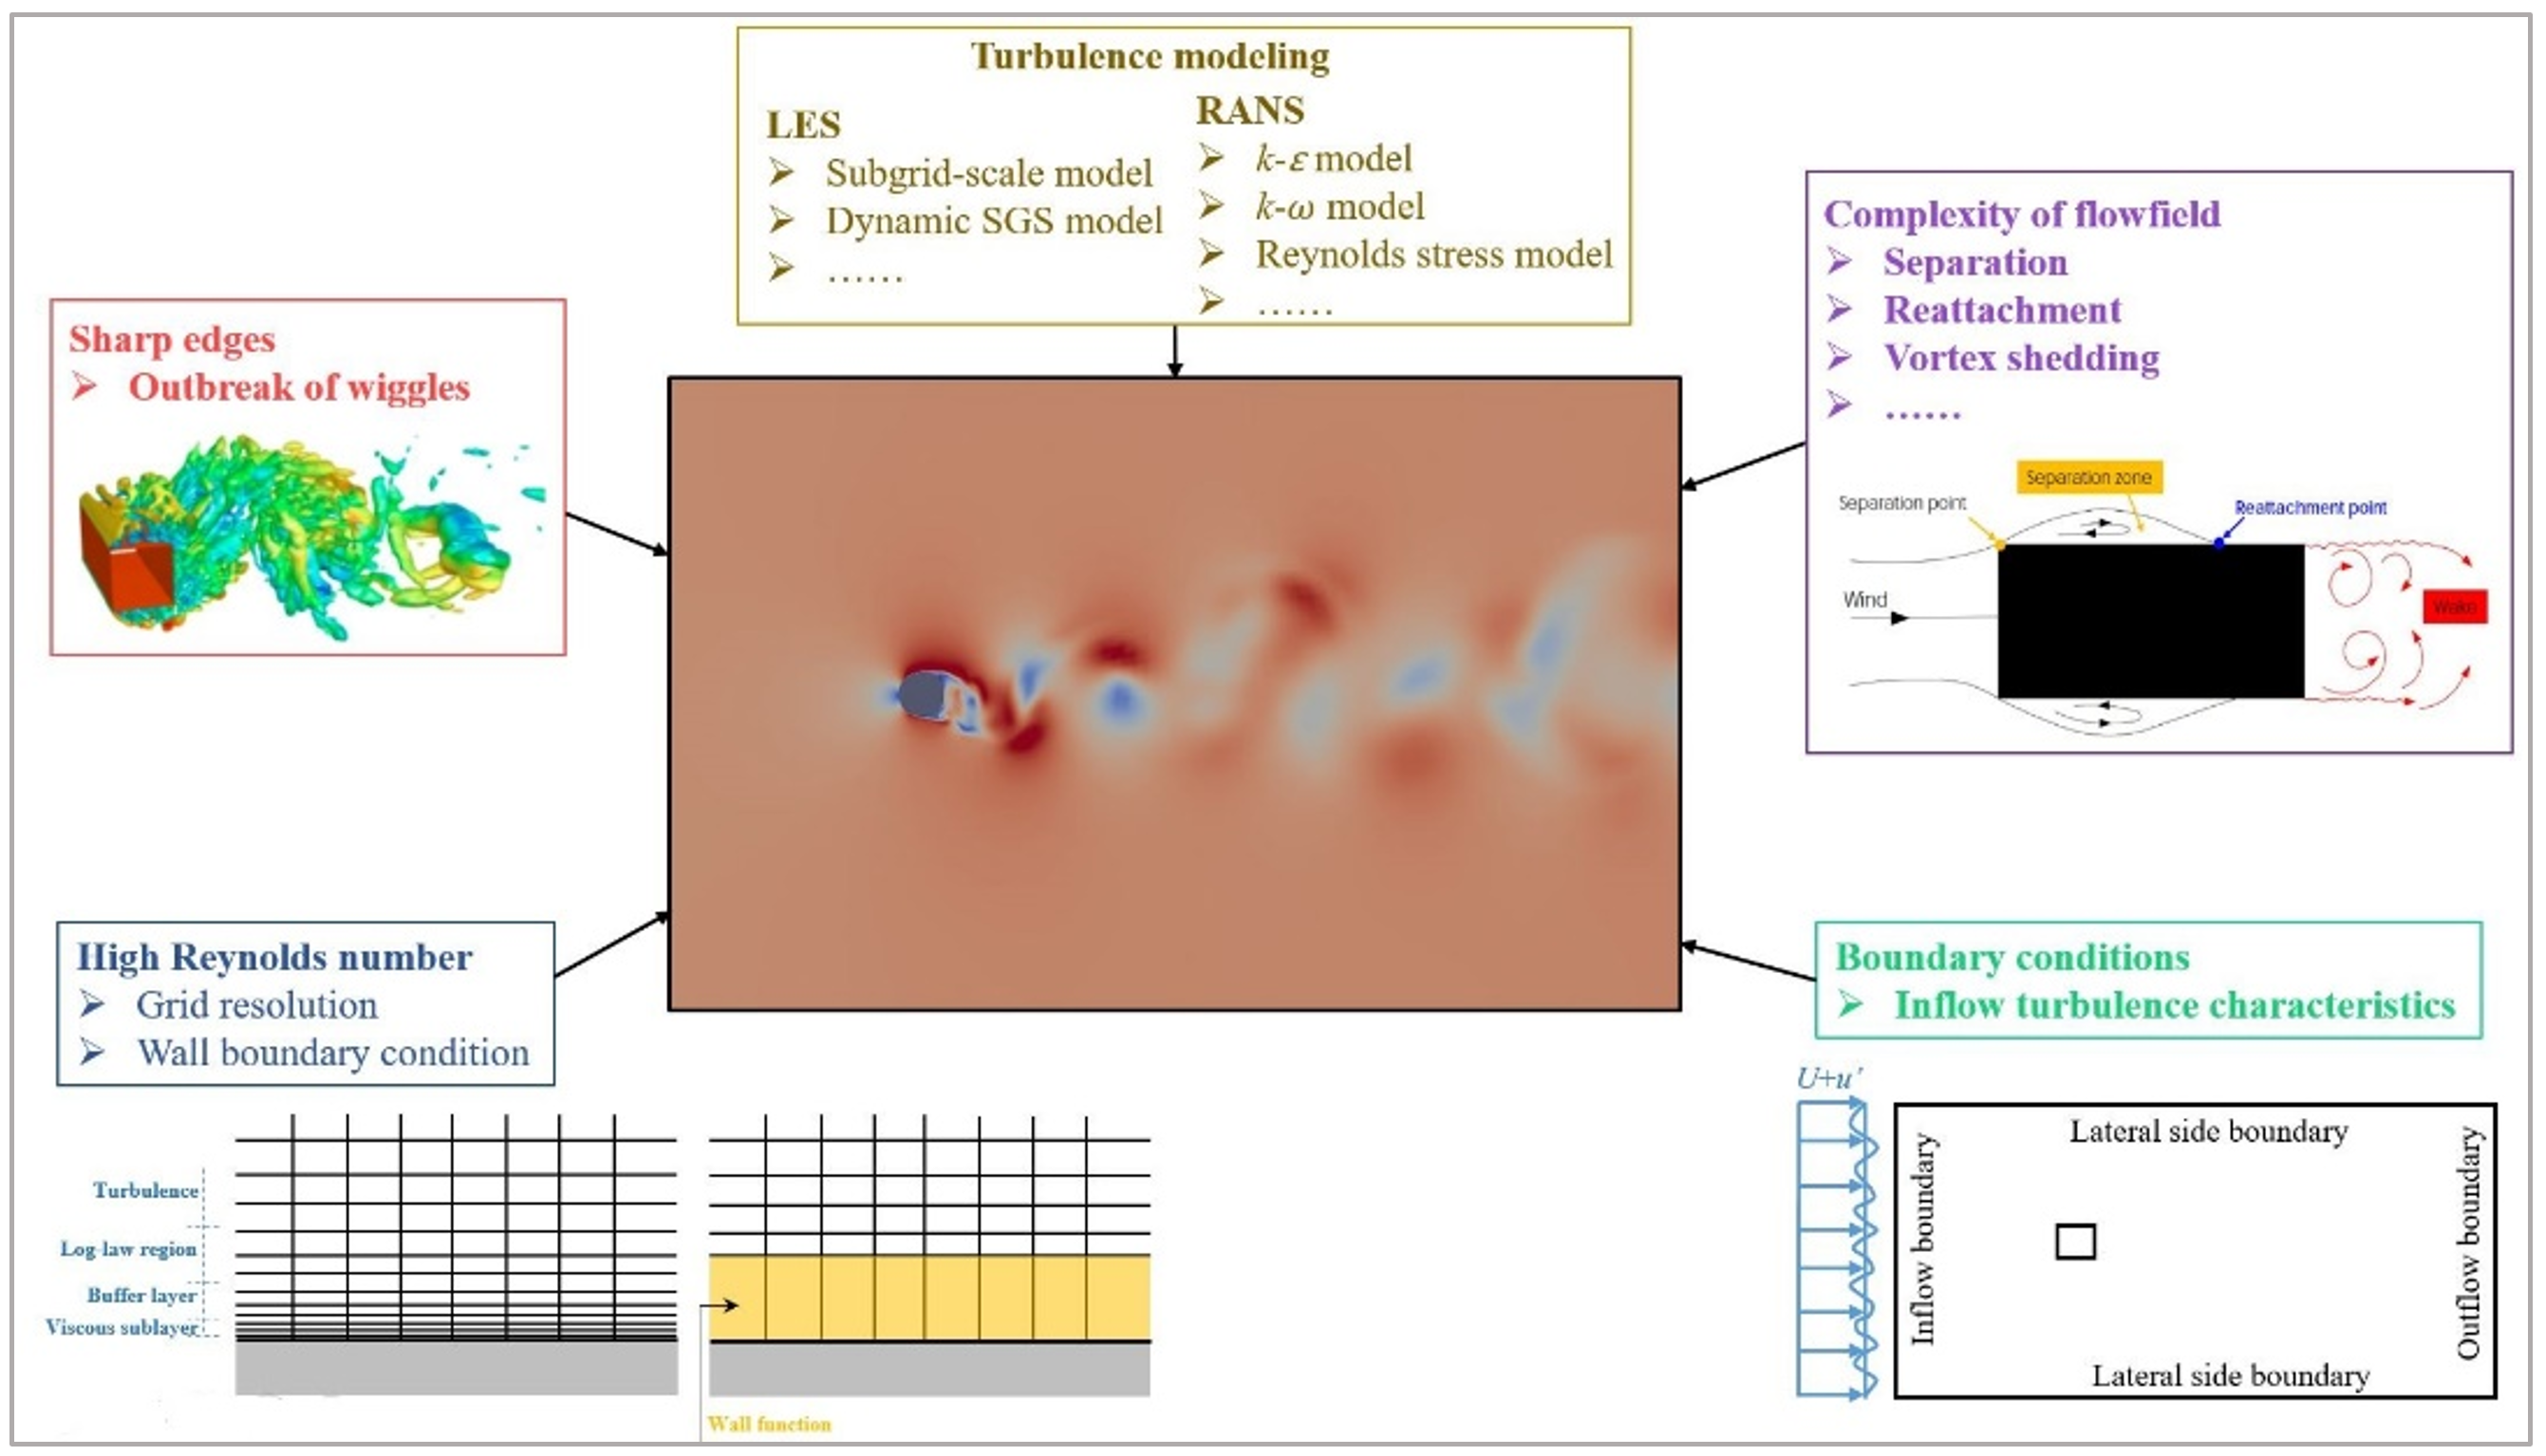
\includegraphics[width=1.0\textwidth, angle = 0]{Figures/DigitalAnalogModeling.png}
    \caption{Schematic of a digital analog of modeling flow around structures in a wind tunnel \citep{ding2018aerodynamic}}
    \label{fig:cfdWind_DAModeling}
\end{figure}

In computational wind engineering (CWE) applications, generation of inflow turbulence satisfying prescribed mean-velocity profiles, turbulence spectrums, and spatial and temporal correlations is of great importance for accurate evaluation of wind effects on buildings and structures. Several methodologies have been proposed for this purpose, which can be classified into three general categories: precursor simulation methods, recycling methods, and synthetic methods. Compared with precursor simulation and recycling methods, the synthetic methods, in general, offer a more practical and relatively efficient approach to generate inflow turbulence. Research activities on synthetic turbulence generation have been vigorous over the past several decades and have branched out into several categories of techniques \citep{wu2017inflow}, including the synthetic random Fourier method \citep{kraichnan1970diffusion, hoshiya1972simulation}, the synthetic digital filtering method \citep{klein2003digital}, and the synthetic eddy methods \citep{jarrin2006syntheticeddymethod}. SimCenter's TinF inflow simulation tool offers a range of inflow simulation schemes for the user to select (\citeprgm{Tinf}). A comprehensive modeling approach for the neutral atmospheric boundary layer: consistent inflow conditions, wall function and turbulence model closure for a RANS based modeling are detailed in \citep{parente2011comprehensive}.

One of the challenges with inflow simulators is the decay of synthetic turbulence as we move from the inflow plane to the location of a building in the simulation domain (3, 4). One of the approaches involve an iterative approach through trial and error, or establishing a transfer function of the decay and embedding that in the simulation scheme. Alternatively,  implementing an optimization to calibrate the inflow parameters is one way to circumvent this challenge and ensure that the correct turbulent statistics are obtained at the location of interest \citep{lamberti2018optimizing}. Besides, there are continued efforts to develop improved inflow generation methods that could further reduce the decay  \citep[e.g.,][]{bervida2020synthetic}. Independent of the choice for the inflow generator, the need to first run an ABL simulation and verify whether the correct turbulence statistics are achieved at the location of interest, similar to the calibration of the flow in a wind tunnel is important.


\section{Computational Details and Post-Processing}
\label{sec:resp_cfd_wind_flow_modeling}

The following discussion addresses computing time for simulation, and how it is influenced by several steps involved in the simulation process. For example, the computing time depends on: (1) the choice of numerical algorithm and data structure; (2) linear algebra solvers and criterion prescribed for interactive solvers; and (3) discretization parameters, such as mesh quality, mesh size, time step; hardware, vectorization, and parallelization. The quality of simulation results depends on: (1) the mathematical model and underlying assumptions; (2) types of approximations implied; and (3) stability of numerical scheme in terms of mesh, time step, error indicators, and iteration stopping criterion. Some of these features operate in isolation while others operate in combination, which influences both the time taken for the simulation and its quality. These processes should be revisited when there is a need to enhance the quality of simulation and/or to reduce the time needed for simulations. Machine-learning tools--such as supervised, unsupervised learning, reinforcement learning, and deep learning--offer exciting avenues to learn from the simulations, help classify regions of similarity and create predictions for future simulations \citep{kareem2019generalized}.

Once the simulations are complete, one needs to process data. This also entails the calculation of derived quantities, e.g., statistics of velocity or pressure fields; integral parameters, e.g., drag and lift coefficients, building response and their spectral characteristics; local zooming for a further look at a region of simulation exhibiting features of potential interest; visualization of data in space and time, a real-time portrait of flow features, digital version of analog flow visualization using smoke in wind tunnels, overall systematic analysis of data using statistical and signal processing tools and debugging, verification and validation of CFD models, and assessing the role of uncertainty.

\section{Verification and Validation}
\label{sec:resp_cfd_wind_flow_modeling}

Wind-tunnel validation of CFD-based simulations often serves as the final step in the process. The progressive reduction of uncertainty \citep{roache1998verification} is the only practical way to ensure any kind of confidence in a given CFD simulation. This calls for vigorous validation \citep{aiaa1998guide}, just as in any other complex numerical simulation. In particular, due to limited analytical solutions being available for simple flows only, CFD validation must be carried out through high-fidelity experimental testing. For this reason, experimental validation often becomes the essential step in ensuring the reliability of CFD simulations \citep{oberkampf2004verification, oberkampf2008verification,roy2011comprehensive}. This is particularly true in computational wind engineering, where the CFD simulation of a bluff body, like a tall building, immersed in an atmospheric boundary layer is often validated through specific boundary-layer wind-tunnel tests \citep{yu1998parametric,yu2013simulation}.

It should be noted that many CFD studies seem to lack a thorough validation process, i.e., grid convergence studies are rarely carried out, and, in general, detailed flow field results are missing. The general lack of code verification, discretization scheme selection, turbulence modeling, mesh quality, and sampling time for statistical analysis, etc., adds more uncertainty. It should be observed, however, that this process is by no means simple and will, in general, be far more involved than the validation of channel or pipe flow, for instance, for a number of reasons including: (1) most experimental wind tunnel tests carried out on civil engineering structures are not exhaustive enough to allow a truly complete CFD validation; (2) the geometric configurations of the bluff bodies tested in wind tunnels are often too complex for an unsteady CFD analysis; and (3) the high Reynolds number in wind tunnel testing also adds difficulties in performing a systematic grid convergence study.

\section{Future Directions}
\label{sec:resp_cfd_wind_flow_modeling}

\paragraph{UQ in CFD modeling} Uncertainties in CFD modeling are primarily associated with the uncertain inflow boundary conditions representing the inherent variability of atmospheric flows and model-form uncertainties originating from the turbulence modeling assumptions applied to the unresolved small-scale turbulent eddies. These sources of uncertainties should be appropriately accounted for, and their impact on the predictive capabilities for the aerodynamic quantities need to be carefully examined since they may impact the aerodynamic loading characterization in CFD modeling. UQ in CFD modeling involves the quantitative estimation of both the inflow and model-form uncertainties, and their resulting impact on the aerodynamic Quantities of Interest (QoIs). Techniques for UQ and uncertainty propagation including Monte Carlo simulations, polynomial chaos, and Gaussian process regression have been explored in many engineering problems as non-intrusive approaches that use solution samples to numerically estimate the output functions \citep{beran2017uncertainty}. An efficient UQ approach that quantifies the effect of coupled inflow and model-form uncertainties would allow propagation of uncertainties to the aerodynamic QoIs. Recent applications of UQ to CFD simulations can be found in \citep{gorle2015quantifying} that utilizes an interval-based approach, while \citep{ding2019inflow} introduced a surrogate model-based scheme. Advances in data-driven approaches are leading to other schemes like DNN for UQ  \citep[e.g.,][]{ling2016reynolds, luo2019deep}].

\paragraph{Multi-fidelity modeling} CFD evaluations can feature both the high-fidelity models, which are accurate yet expensive and the low-fidelity models that are computationally efficient but can produce large modeling errors. RANS and its variants are currently the workhorse of CFD \citep{kareem2017computational} as the computational requirements are modest, but because its accuracy is compromised in separated flow regimes, it is viewed as low fidelity. LES solves the filtered NS equations at large energy-containing scales and relies on modeling to resolve the smaller more universal subgrid scales. The results thus offer a higher fidelity compared to RANS, but at an additional computational effort. Therefore, the simulation data may involve data sources of multiple fidelities with different computational costs.

In an attempt to blend the variable-fidelity information source, multi-fidelity surrogate modeling is an attractive avenue that utilizes hierarchical surrogate models relating low-fidelity (RANS) to high-fidelity (LES) models to obtain high-quality predictions with a computational effort comparable to RANS. Multi-fidelity surrogate modeling has been successfully applied to a host of engineering problems, including beam design, using finite-element analyses with variable mesh sizes \citep{leary2003knowledgebased}, optimization of a transonic aircraft wing with two levels of CFD fidelity \citep{forrester2007multifidelity}, and rotor bade design based on the code with simplified aerodynamics, as well as high-fidelity numerical simulations \citep{collins2008multifidelity}, etc. Therefore, a multi-fidelity surrogate modeling approach in the aerodynamic shape-optimization framework that involves data from sources of both RANS and LES simulations would offer superior surrogates from the context of enhancing the model accuracy as well as maintaining low computational demand.

\paragraph{Fusion of Machine Learning and CFD} As discussed earlier in this section, the CFD-based simulations are computationally very demanding especially with the desired level of fidelity despite recent advances in the computational resources. Recently, the focus in the CFD area is on the fusion of data-driven approaches to enhance the computational times and accuracy of simulations \citep{kutz2017deep, ling2016reynolds, kareem2020emerging}. Using DNNs as a surrogate model to predict CFD simulation results is also a promising future direction. So far relevant studies for Reynolds stress modeling using DNNs, CNNs for flow prediction, or physics-informed neural networks (PINN) which have gained a considerable attraction are applied to solve simple flow patterns at low or moderate Reynolds numbers. [e.g., \citep{tompson2016accelerating, liu2020iterative, mao2020physics}]. This deep-learning-based approach can be also based on experimental data or an integrated experimental and computational simulation framework \citep{luo2019deep, luo2020bayesian}. Others have involved machine learning as a CFD closure model, in which based on representative datasets closure model parameters are extracted and embedded in the flow solver to enhance the quality of simulations. Similarly, machine learning models are being developed to model errors in e.g., RANS or LES based prediction compared to DNS data. \citep{ding2018multifidelity} used a similar surrogate model to account for the discrepancy between RANS and LES simulations of shape optimization of buildings. This approach also facilitates UQ in such an exercise \citep{ding2018multifidelity, ding2019inflow}. Furthermore, machine learning approaches can be used as ``wrappers'' around existing toolsets to enhance predictive capabilities. Other applications involve invoking the concept of digital twins for the exploitation of computational physics data, consisting of using machine learning to enlarge the simulation databases to cover a wider spectrum of operational conditions and provide quick response directly on the field \citep{kareem2020emerging, molinaro2021embedding}. The resulting product from this hybrid physics-informed and data-driven modeling may be referred to as Simulation Digital Twin. A recent example of CFD, machine learning, sensing and actuation of a dynamic building façade shows an example of how the fusion of these technologies can offer a viable platform to manage autonomously the profile of a building façade under varying wind environments \citep{ding2020tall}. 
